%!TEX root = ../thesis-summary.tex

\section{Pulsarcast}
\label{section:pulsarcast}

Pulsarcast is a peer to peer, pub-sub, topic-based system focused on
reliability, eventual delivery guarantees, and data persistence. We seek this
while not fully compromising the scalability given by the decentralised nature
of our architecture. Looking through our related work, it became clear that few
fully decentralised solutions exist that try to provide this kind of
guarantees. Yet, if we carefully look at the most popular and widely adopted
centralised pub-sub solutions, it is clear that most of them heavily rely and
depend upon these same guarantees. 

We opted for the more straightforward topic-based subscription model given
that, in our view, a well structured and implemented topic-based model is more
than enough for a significant percentage of our use cases. In the end, we
compromise a bit of the expressiveness of the system in order to avoid bringing
more complexity in, something we believe will pay off.

Pulsarcast is a fully decentralised solution, which means that each node plays
a crucial part in fulfilling the system's purpose, delivering events and
ensuring their dissemination. Conceptually speaking, Pulsarcast provides four
methods for clients and applications to interact with the system, create a
topic, subscribe to a topic, unsubscribe from a topic and publish an event in a
topic. From a broader perspective, Pulsarcast relies on two overlays to fulfil
its needs. Kadmelia DHT, already employed by IPFS and used by
Pulsarcast for peer discovery, content discovery and to bootstrap our other
overlay, the Pulsarcast own overlay. The Pulsarcast overlay is actually a set of
different overlays or, as we call it, dissemination trees.  These trees are on
a per topic basis and are the critical factor in the way we disseminate
information across our decentralised network.  Figure
\ref{fig:pulsarcast-overlays} illustrates the multiple overlays in action.

\begin{figure}[hb!]
  \centering
  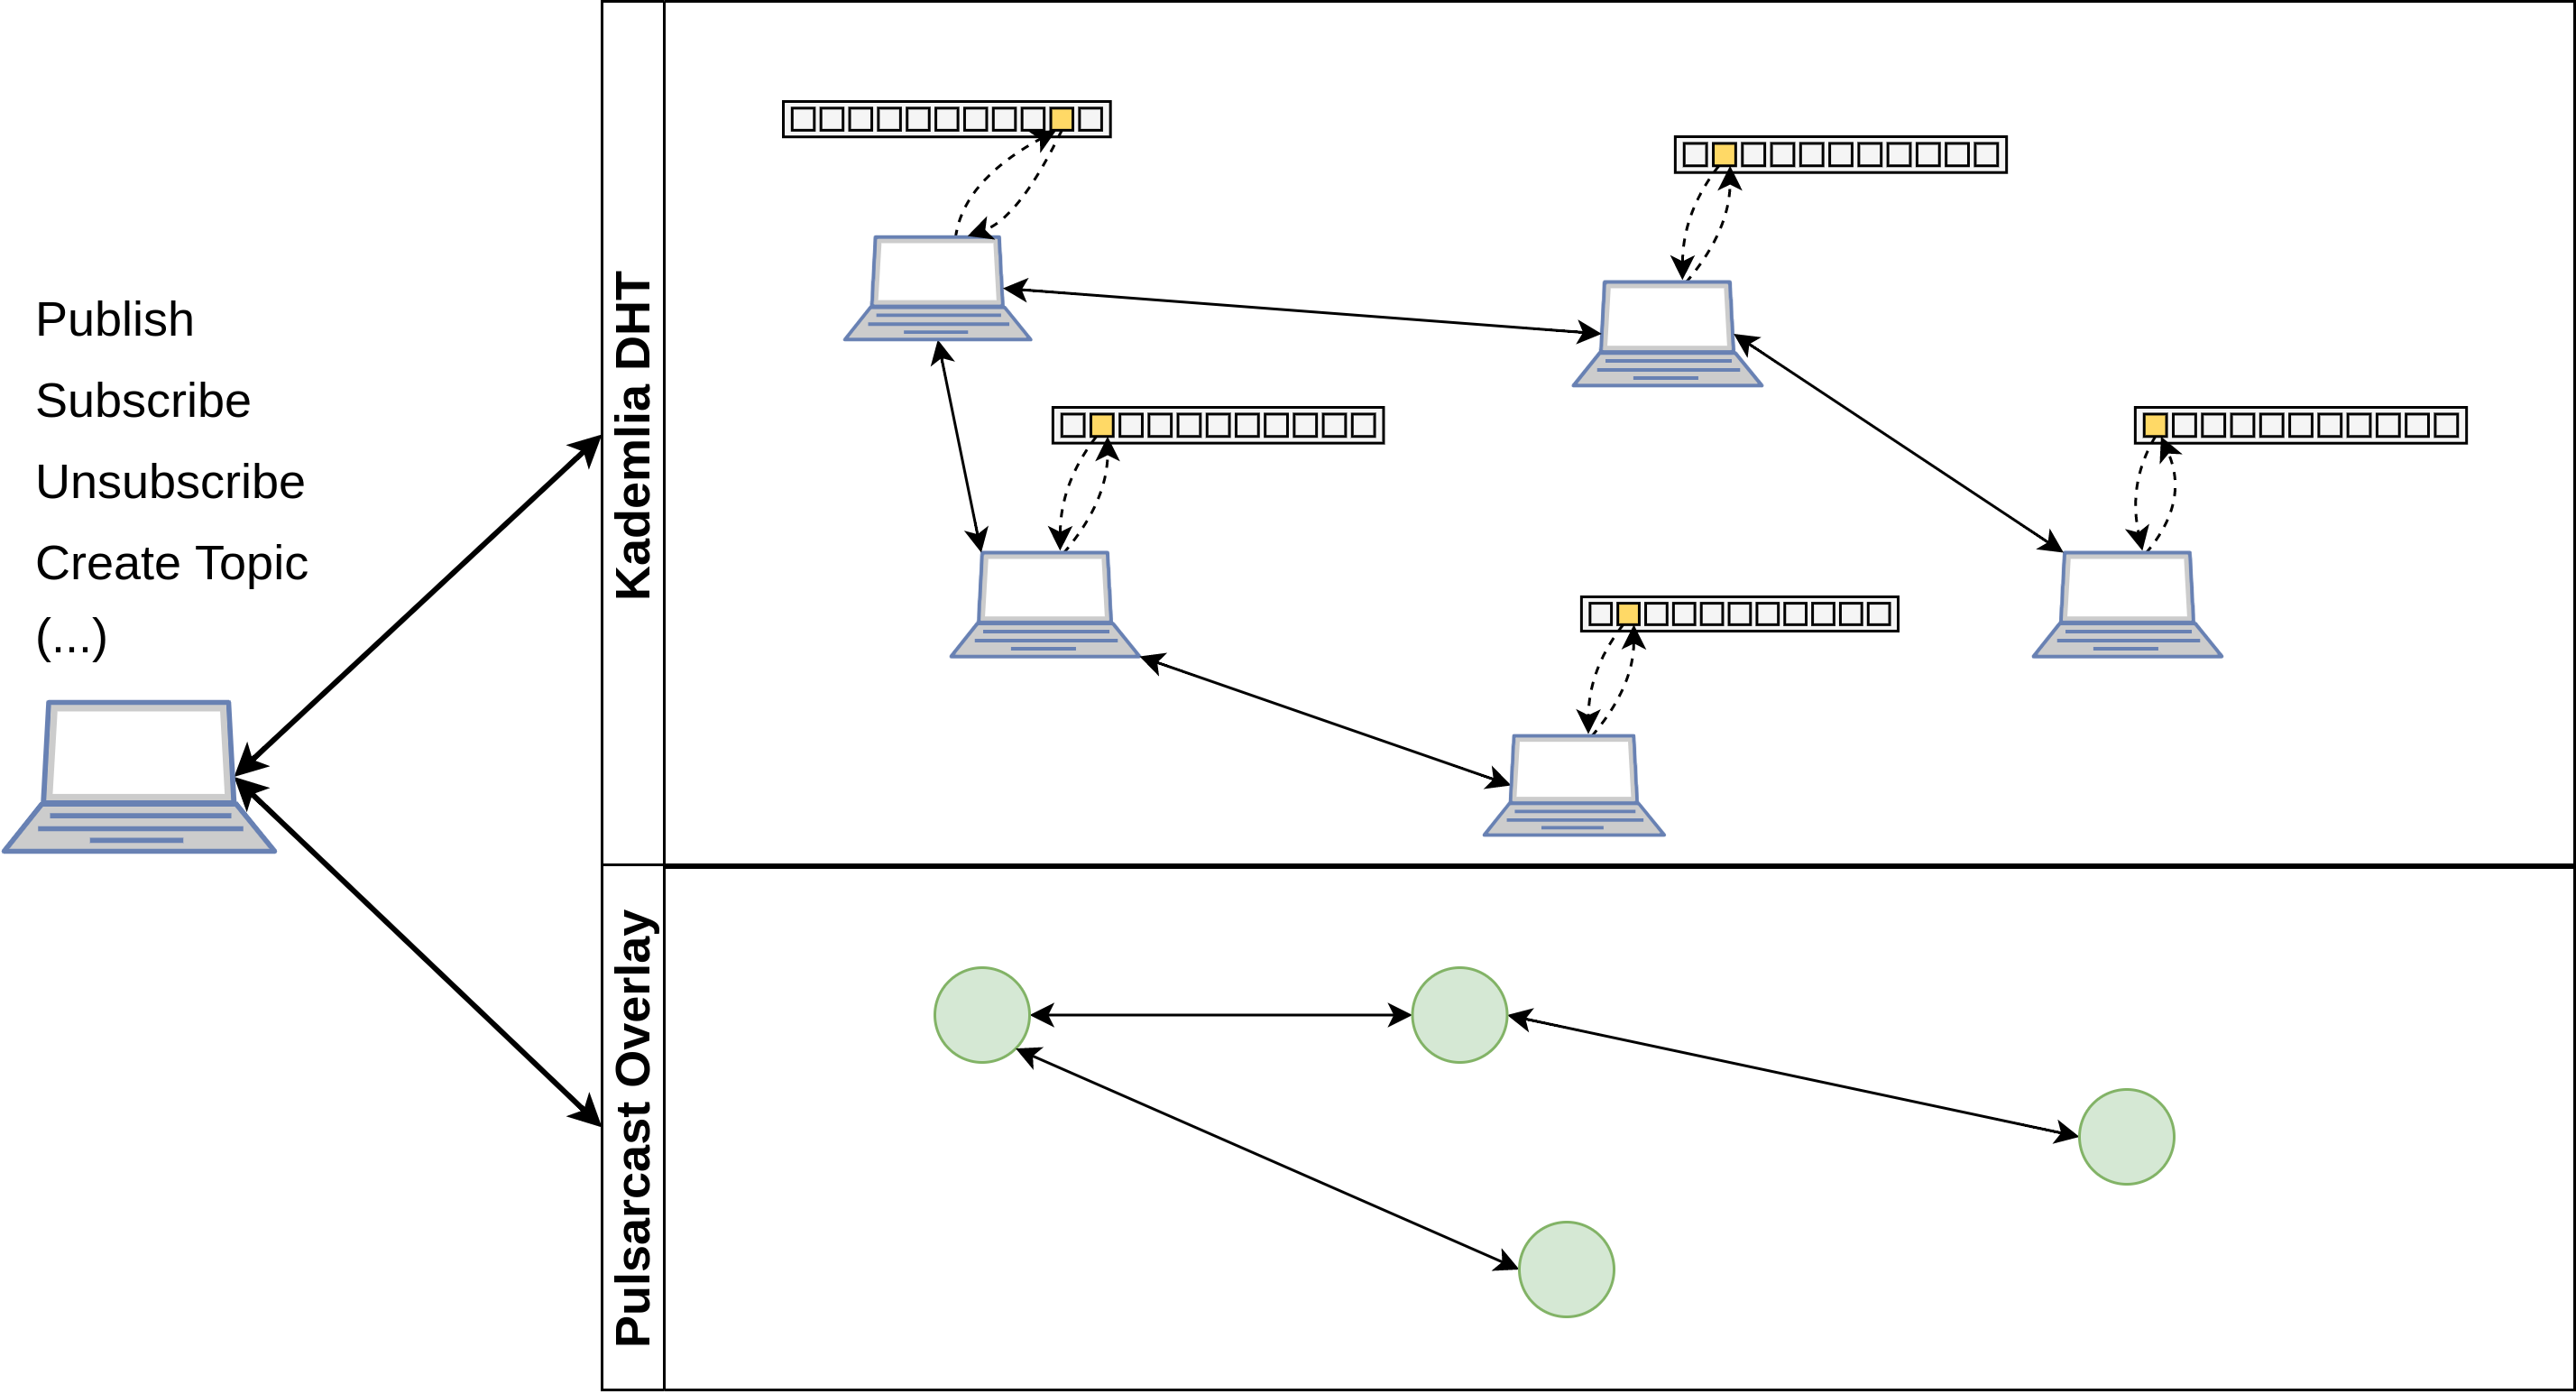
\includegraphics[width=0.48\textwidth]{img/pulsarcast-overlays.png}
  \caption{Representation of the Pulsarcast overlays}
  \label{fig:pulsarcast-overlays}
\end{figure}

The subscription model followed by Pulsarcast is a topic based one, but still
allowing for some expressiveness through the usage of sub-topics to enable more
complex structures. When a peer publishes an event or creates a new topic a set
of the overlays described is used accordingly. For Pulsarcast, both of these
actions, happen to take a similar course. That is because the system views
these pieces of information (or descriptors as we call it) as fairly similar,
given their importance. Figures \ref{fig:pulsarcast-descriptor-creation} and
\ref{fig:pulsarcast-descriptor-query} provide an overview of how the flows for
creating this information and for accessing it look like.

\begin{figure}[hb!]
  \centering
  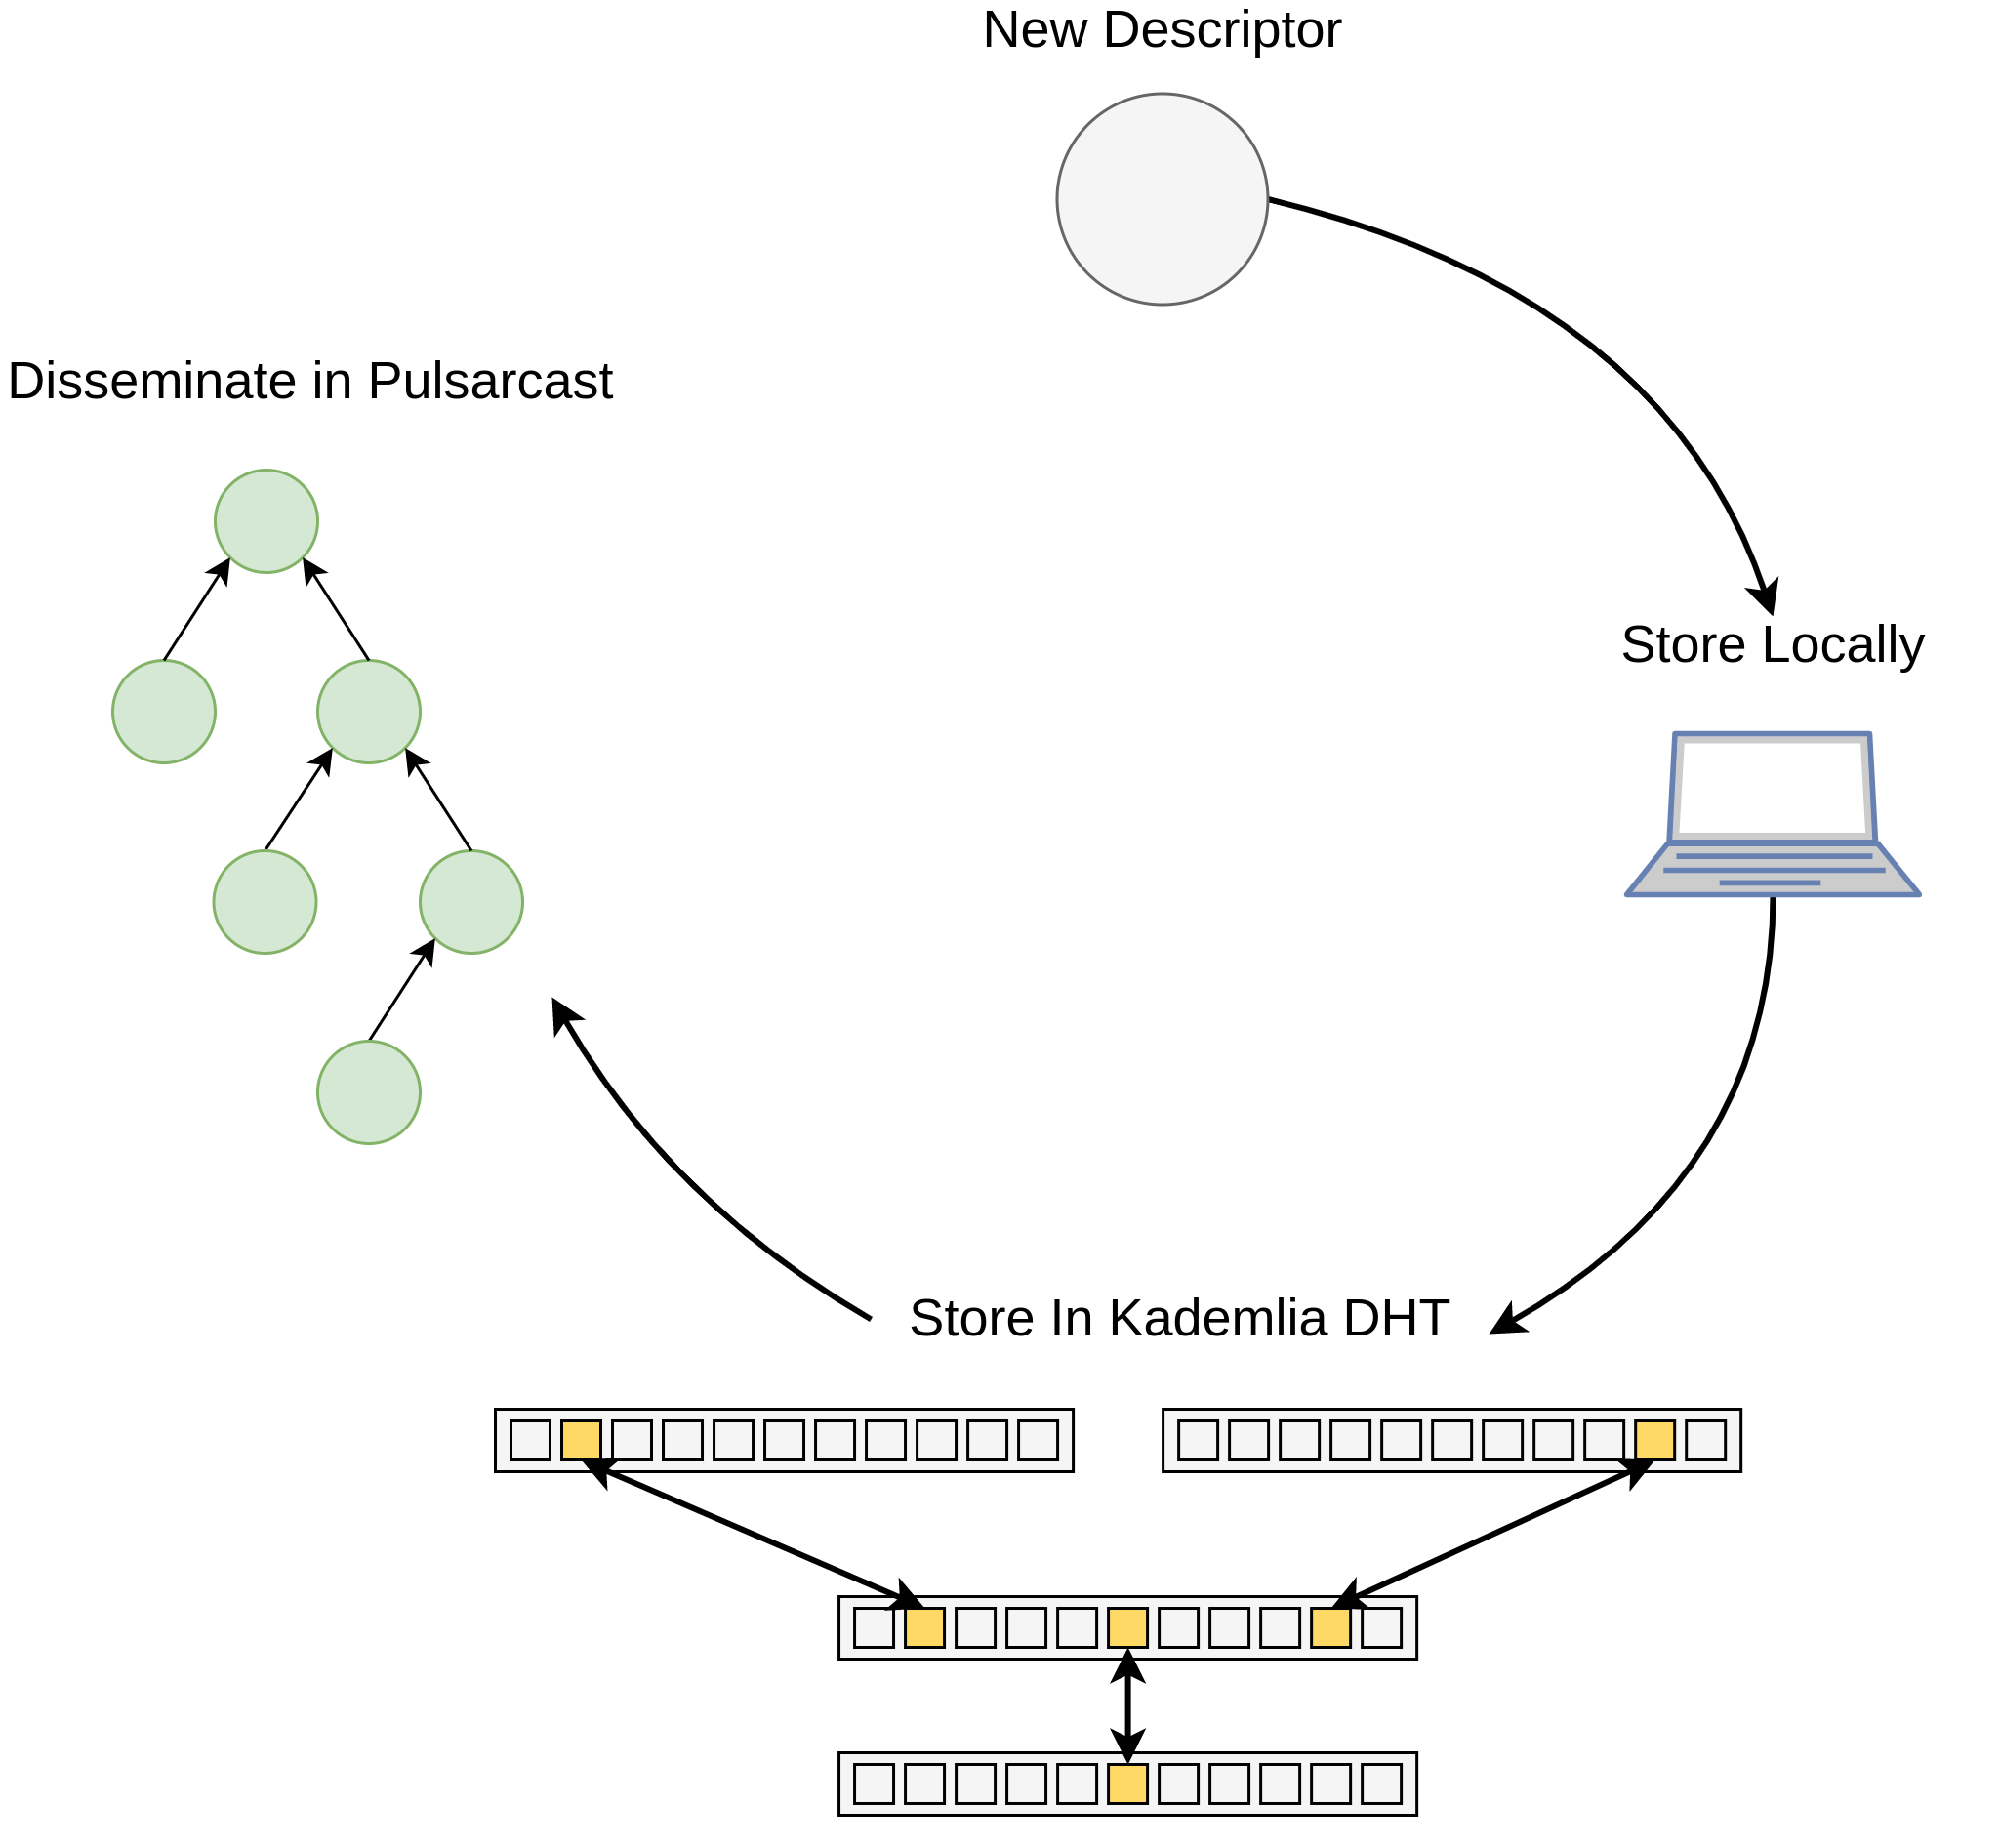
\includegraphics[width=0.4\textwidth]{img/pulsarcast-descriptor-creation.png}
  \caption{Flow for creating a new Topic/Event descriptor}
  \label{fig:pulsarcast-descriptor-creation}
\end{figure}

\begin{figure}[tb!]
  \centering
  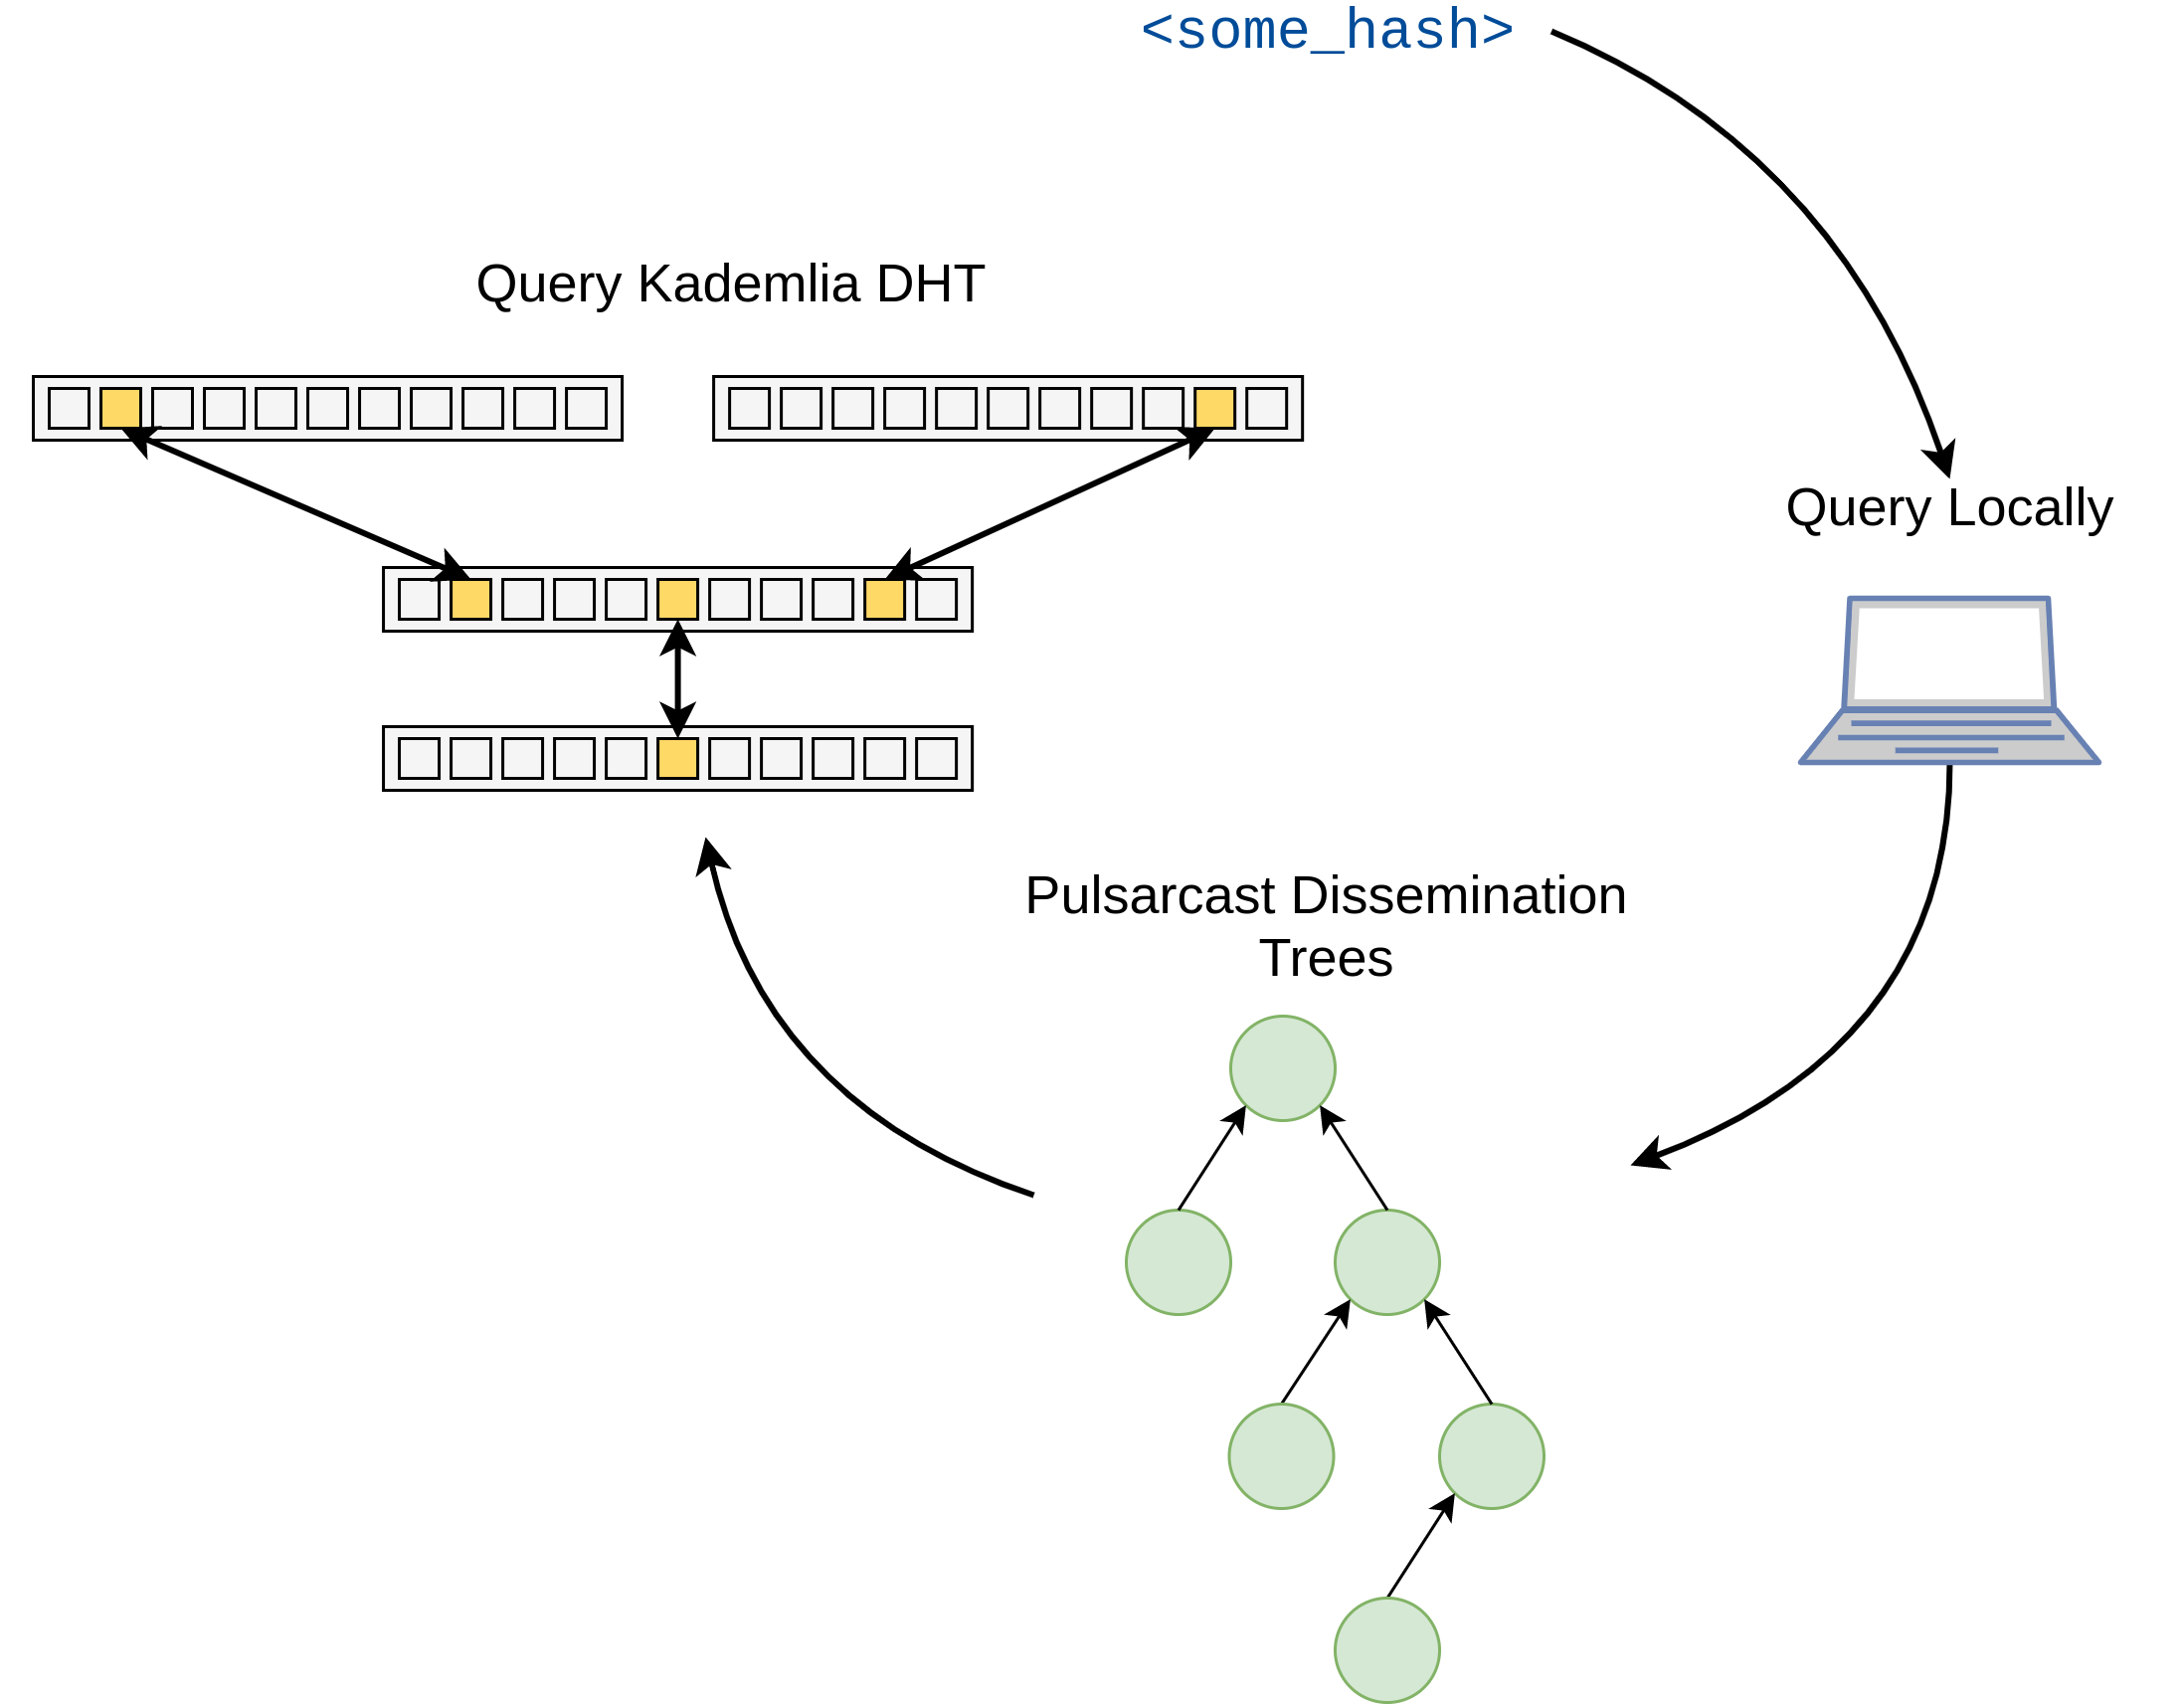
\includegraphics[width=0.4\textwidth]{img/pulsarcast-descriptor-query.png}
  \caption{Flow for querying a Topic/Event descriptor}
  \label{fig:pulsarcast-descriptor-query}
\end{figure}

Pulsarcast's goal is to give users and any applications built on top of it the
reassurance that events reach their destination and that they can rebuild as
much of the event or topic history as they see fit. As such, we doubled our
efforts to persist and propagate data. Every topic and event is stored in the
Kadmelia DHT before being forwarded through the topic dissemination
trees.  This ensures the data is persisted by a set of nodes (that might even
be extraneous to the topic at hand) and anyone is later able to fetch the data
using only the DHT if they want to. Afterwards, we forward the data
through the appropriate dissemination trees previously built.
Currently, every node participating in the data transmission through the
dissemination tree stores it indefinitely, although it is something due to
being changed in a later revision of our protocol (e.g. by means of predefined
global or topic-specific temporal time-out, or by a special message per topic
flushing all past events up to a specific one). On the other hand, when someone
wants to fetch a piece of data (a topic or an event) it starts by performing a
local search in the system, it might have been something that the node has run
through when forwarding events across their dissemination trees. If this fails,
though, a query to the DHT is in order.
